\chapter{\label{chp:beams} Neutrino Beams}

Direct measurements of neutrinos have two parts: a source of neutrinos, and a detector to observe them.  The most precise experiments required detailed knowledge of the workings of both the source {\em and} the detector.  This chapter describes the important components of the Fermilab accelerator based neutrino beams.  The Booster Neutrino Beam (BNB) is relevant to the Fermilab Short Baseline Neutrino Program, in Chapters~\ref{chp:sbn} and \ref{chp:systematics}.  The Neutrinos from the Main Injector (NuMI) beam is relevant for the \argoneut experiment in Chapter~\ref{chp:emshowers}. 

\section{Accelerator Based Neutrinos}

A popular source of neutrinos in modern experiments are the neutrinos from accelerator complexes.  As of the writing of this thesis, there are three active neutrino beams: two at Fermilab \cite{Adamson:2015dkw, AguilarArevalo:2008yp}, and one in Japan \cite{Abe:2014oxa}.  Compared to other sources of neutrinos, accelerator based neutrinos offer some advantages.

First, neutrino beams made at accelerator complexes are designed, and not a by-product of other circumstances.  This means that the design of the beam is often optimized for physics goals, in particular by tuning the energy spectrum and energy range of the neutrino beams.  Combined with intelligent positioning of detectors, accelerator neutrino beams can be optimized to probe a vast range of oscillation signals.

The NuMI beam, described below, was designed to have three modes of running to cover an entire energy range from 1 to 20 GeV neutrinos.  In general, accelerator based neutrino sources are crafted to build neutrino beams that will allow the neutrino experiments in the beam to maximize their physics output.

Another advantage to neutrino beams at accelerators is the pulse structure of the beam.  Since accelerators, like Fermilab, make neutrino beams by colliding bunches of protons with a target material, the timing of the proton bunches provides a natural time structure to the neutrino beams.  Downstream detectors can, using sufficiently time-sensitive detection material, ``time-in'' to the neutrino beam pulses to reject non beam backgrounds.  For experiments on or near the surface, this is exceptionally important for rejecting cosmic backgrounds.

\section{Fermilab's Accelerator Complex}

At Fermilab, where two of the three active neutrino beams originate, much of the physics program is derived from the use of the proton beam that Fermilab produces.  All of the proton beams, regardless of destination, start in the same location.  A bottle of hydrogen provides a source of protons for the entire accelerator complex.  In batches, some of the hydrogen atoms are given a negative charge by the addition of an electron, and these electrons are pushed into the Linear Accelerator (LINAC) at Fermilab with 750 KeV of energy (via a Cockroft-Walton generator).  The LINAC accelerates the protons to 400 MeV, and at the end of the LINAC the protons enter the Booster, a synchrotron.  Before entering the Booster, the electrons are knocked off of the H$^-$ ion to ensure that only protons enter the downstream accelerator system.  Over the course of thousands of rotations around the Booster, the protons are accelerated to 8 MeV of kinetic energy.

The Booster can nominally operate at 15 Hz, though is generally run at lower frequencies.  Future upgrades to Fermilab's accelerator complex involve running the Booster at it's maximum rate to produce as many protons as possible.  From the Booster, protons can be extracted to the Booster Neutrino Beam target, described below (Section~\ref{sec:bnb}).  The majority of protons, however, enter the Main Injector to be accelerated to higher energies.  The Main Injector can accelerate protons to 120 GeV.

At the time of writing, the majority of the protons from the main injector are used in the NuMI beam (Section~\ref{sec:numi_beam}), while some are used for fixed target experiments and test beams (beams made of pions or other particles, generally secondary or tertiary beams from the proton beam).  At the time of the data collected for this analysis, however, some of the protons from the Main Injector were used to produce anti-protons for the Tevatron, and some were injected into the Tevatron directly.  In the future, it's excepted that a large fraction of protons will be used for the muon campus (for mu2e and g-2 \cite{Bartoszek:2014mya} \cite{Grange:2015fou}), and further protons will be used for the LBNF Neutrino Beam \cite{DUNE}.

\section{Booster Neutrino Beam}
\label{sec:bnb}

The Booster Neutrino Beam (BNB) is Fermilab's lower energy neutrino beam, and the primary beam of \MB, \uboone, and the Short Baseline Neutrino Program (see Chapter \ref{chp:sbn}).  The BNB is one of the most well understood, extensively studied neutrino beams in existence, and has been running since the \MB experiment and is expected to run until past 2020.

\subsection{Booster Neutrino Beam History}
The BNB was designed for, and by, the \MB collaboration.  \MB was a Cherenkov style detector, searching for electron neutrino appearance.  Because the primary background for \MB was photons from neutral pion production in the detector, which come from higher energy neutrinos, the BNB flux was designed to suppress neutrinos with energy above $\approx$ 1 GeV.

The origin of the BNB is 8 GeV protons (8.89 GeV/c momentum) from Fermilab's Booster complex.  These protons are transported to a Beryllium target, encased in a magnetic focusing horn.  The protons collide with the Be and produce hadrons within the target, which are focused into the forward direction by the focusing horn.  The hadrons enter a decay pipe of 50 meters, where they decay in flight into lighter particles including neutrinos.  At the end of the decay pipe is a beam stop to prevent all particles (except neutrinos) from proceeding.  A schematic of the proton entry, horn location, decay pipe and beam stop are shown in Figure~\ref{fig:mb_target_schematic}.

\begin{figure}[tb]
  \centering
  \includegraphics[width=\textwidth]{beams_figures/mb_target_schematic}
  \caption[BNB Target Schematic]{The Booster Beam target hall and decay pipe.  Protons enter from the left, and hadrons decay in the decay pipe for up to 50m before the beam stop.  \MB, \uboone, and the other SBN experiments are to the right. Figure from \cite{AguilarArevalo:2008yp}}
  \label{fig:mb_target_schematic}
\end{figure}

The batches of protons delivered to the Booster target are pulsed, typically at a rate not more than 5 Hz, and each bunch is approximately 1.6$\mu$s in duration.  For downstream experiments, such as \MB and the SBN Program, the ability to resolve interactions in the detector on the time scale of 1.6 $\mu$s is extremely useful for rejecting out-of-beam-time cosmics.  

Each bunch of protons from the Booster typically contains approximately 4e12 protons.  These protons collide with the Beryllium target, which is 71 centimeters long and made from seven segments of Beryllium.  This length corresponds to 1.7 interaction lengths for the protons, meaning that just over 80\% of the protons interact in the target material.  The number of protons on target is measured upstream of the target by two magnetic toroids, and the uncertainty on the number of protons delivered is on the order of 1-3\% typically.

Upon interacting, the protons produce lighter hadrons such as pions and kaons.  The spectra of produced hadrons is the source of the largest uncertainty in the Booster Neutrino Beam, and is discussed in more detail in Section~\ref{section:flux_uncert}.  The hadrons produced by the protons at the target are focused with the magnetic horn which produces an azimuthal, pulsed magnetic field in time with the proton delivery.  The primary source of the neutrinos in the BNB is from decay in flight pions, though there is significant contamination from kaon decay and muon decay (where the muons are also the product of pion decay).  The kaons and muons also produce a contamination of electron neutrinos in the primarily muon neutrino beam, and this flux of electron neutrinos is the primary background in the Short Baseline Neutrino Program's \nue appearance analysis (see Section~\ref{subsection:event_reco}.

The estimation of the flux, by neutrino type and by originating particle, at the \MB location can be seen in Figure~\ref{fig:mb_flux_nu}.  This estimate of the flux is produced with a sophisticated Monte Carlo simulation, discussed in detail in \cite{AguilarArevalo:2008yp}.  However, the general procedure is:

\begin{enumerate}

\item{Define the beamline geometry, including the shape, location, and composition of the components of the BNB.  This includes the target, magnetic horn, decay pipe and beam stop as well as the other minor parts.  The simulation attempts to capture the reality of the beam construction as closely as possible.  A graphical representation of the magnetic focusing horn can be seen in Figure~\ref{fig:mbhorn}.}

\item{Generate protons in the simulation that match the expected protons from the beam, accounting for the optical effects of the beam upstream of the target.}

\item{Simulate the interaction of protons in the target and surrounding material.  Substantial effort was made by the \MB collaboration to constrain this step of the simulation, as it is the primary source of systematic uncertainties in the beam model.  Dedicated experiments, such as HARP \cite{Catanesi:2007ab} and BNL E910 \cite{Chemakin:2007aa}, are used to constrain pion production and improve the flux prediction, as the uncertainties in pion production dominate the flux uncertainties.}

\item{Propagate particles from the primary interactions using GEANT\cite{Agostinelli:2002hh} to account for energy loss and interactions that change the kinematics of the particles above.  This also includes accounting for the focusing effects of the magnetic horn.}

\item{Identify particles that result in neutrinos at the detector, accounting for branching ratios and kinematic distributions properly.  Statistical boosting techniques are also used, since the solid angle subtended by the neutrino detector is small in the lab frame of the decaying particles.}

\end{enumerate}

\begin{figure}[tb]
  \centering
  \includegraphics[width=\textwidth]{beams_figures/mbhorn}
  \caption[BNB Horn and Focusing Magnet]{The Booster Beam horn and focusing magnet.  Figure from \cite{AguilarArevalo:2008yp}}
  \label{fig:mbhorn}
\end{figure}

\begin{figure}[tb]
  \centering

    \begin{subfigure}[t]{0.5\textwidth}
        \centering
        \includegraphics[height=2in]{beams_figures/mb_flux_nu}
    \end{subfigure}%
    ~ 
    \begin{subfigure}[t]{0.5\textwidth}
        \centering
        \includegraphics[height=2in]{beams_figures/mb_flux_by_type_nu}
    \end{subfigure}
  \caption[\MB Flux]{(Left) Total predicted flux at the MiniBooNE detector by neutrino species with horn in neutrino mode. (Right) Muon neutrino flux by type of original particle. Figure from  \cite{AguilarArevalo:2008yp}}
  \label{fig:mb_flux_nu}
\end{figure}

The work covered in this document does not use the \MB detector at all, however it does leverage the \MB flux calculation machinery to simulate the flux at multiple locations for the Short Baseline Neutrino Program, shown in Figure~\ref{fig:sbn_flux}.  In this light, the discussion of the systematic uncertainties of the flux prediction are left to Section~\ref{section:flux_uncert}.  However, Table~\ref{tab:mb_flux_uncert} is included here to showcase the precision at which \MB constrained the BNB, an accomplishment that future experiments are building upon.

\begin{figure}[htbp]
  \centering
  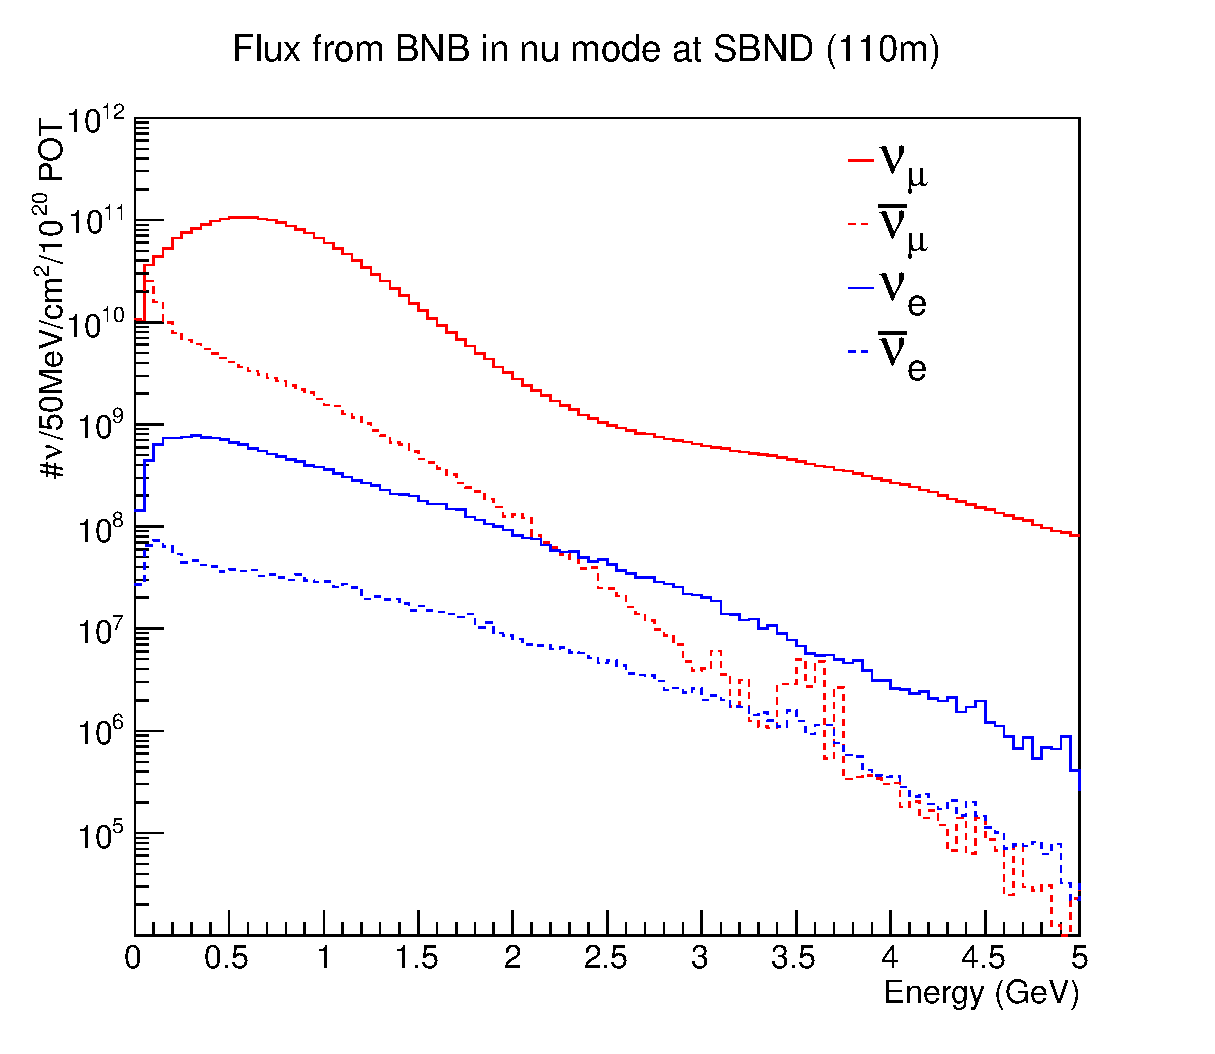
\includegraphics[width=0.45\textwidth]{beams_figures/bnb_flux_nu_100m.eps}
  \includegraphics[width=0.45\textwidth]{beams_figures/bnb_flux_nu_470m.eps}
  \includegraphics[width=0.45\textwidth]{beams_figures/bnb_flux_nu_700m.eps}
  \caption[BNB Fluxes]{The neutrino flux from the Booster Beam at the three locations of the SBN Program.  The flux falls at approximately $1/r^2$, however, the near detector flux is slightly distorted due to its proximity to the decay pipe.}
  \label{fig:sbn_flux}
\end{figure}

\begin{table}[tb]
  \caption{Fractional flux uncertainties, by species of neutrino, from the \MB flux calculation.}
  \centering

  \begin{tabular}{l|rrrr}
  \hline
  \hline
  Source Of Uncertainty & \textbf{\numu} & \textbf{\numubar} & \textbf{\nue} & \textbf{\nuebar}  \\
  \hline
     Proton Delivery        &  2.0\% &  2.0\% &  2.0\% &  2.0\% \\
     Proton Optics          &  1.0\% &  1.0\% &  1.0\% &  1.0\% \\
     $\pi^+$ Production     & 14.7\% &  1.0\% &  9.3\% &  0.9\%\\
     $\pi^-$ Production     &  0.0\% & 16.5\% &  0.0\% &  3.5\% \\
     $K^+$ Production       &  0.9\% &  0.2\% & 11.5\% &  0.3\% \\
     $K^-$ Production       &  0.0\% &  0.2\% &  2.1\% & 17.6\% \\
     Horn Field             &  2.2\% &  3.3\% &  0.6\% &  0.8\% \\
     Nucleon Cross Sections &  2.8\% &  5.7\% &  3.3\% &  5.6\% \\
     Pion Cross Sections    &  1.2\% &  1.2\% &  0.8\% &  0.7\% \\
  \hline

  \hline
  \end{tabular}
  \label{tab:mb_flux_uncert}
\end{table}


\section{Neutrinos from the Main Injector (NuMI Beam)}
\label{sec:numi_beam}

The Neutrinos from the Main Injector (NuMI) beam was conceived of with the MINOS (Main Injector Neutrino Oscillation Search) experiment at a time when neutrino oscillation parameters were not well constrained.  In particular, there were hints that the atmospheric mass splitting was of the order of magnitude of $10^{-3} eV^2$, but more than that was unknown.  Therefore, the NuMI beam was designed to be configurable and to run in multiple modes of running: Low Energy, Medium Energy, and High Energy.  The various energy spectra are shown in Figure~\ref{fig:numi_spectra}.  A comprehensive discussion of the design and operation of the NuMI beam is available in Ref. \cite{Adamson:2015dkw}.  This section will be a very brief summary of some important facts about the NuMI beam.

\begin{figure}[htbp]
  \centering
  \includegraphics[width=0.45\textwidth]{beams_figures/numi_focus_vs_perfect.png}
  \caption[NuMI Energy Modes]{The various energy tunings for NuMI.  The analysis performed for this work is based off of the Low-Energy mode, mainly in anti-neutrino mode.}
  \label{fig:numi_spectra}
\end{figure}

The NuMI target is similiar to the BNB target, above, though it is more complex for several reasons.  First, the distance between the target itself and the focusing horns is adjustable to allow the different running configurations.  Additionally, there are two focusing horns instead of just one.  The first horn, located close to the target, and the second horn, downstream, effectively act as a charged hadron focusing system.  With a higher energy source of protons compared to the BNB, the two horns are necessary to focus the higher energy secondary particles from the target.  Downstream of the target and horn area is the NuMI decay pipe, which is 675m in length.  After the decay pipe there is 240m of rock, followed by the near detector for MINOS.  \argoneut, the detector that collected the data of this thesis, is located in the MINOS near detector hall in between MINOS and Miner{$\nu$}a.
The schematic of the target, horn, and decay pipe are shown in Figures~\ref{fig:numi_horn}.

\begin{figure}[htbp]
  \centering
  \includegraphics[width=0.95\textwidth]{beams_figures/numi_beam_target.png}
  \caption[NuMI Beam Target]{The beam target, horns, and decay pipe are shown for NuMI.}
  \label{fig:numi_horn}
\end{figure}

The NuMI flux is simulated with a FLUKA simulation in a way very similar to the BNB.  It also benefits from the constraints from dedicated hadron production experiments \cite{Nigmanov:2009zz, Alt:2006fr}, and in situ measurements from the detectors along the beam line \cite{Aliaga:2016oaz}.  The flux models in the simulation of the beam are generally accurate to with 10 or 20\%, however experimental constraints and flux tunings can decrease the uncertainty to less than 10\% \cite{Aliaga:2016oaz}.  The flux shown in Figure~\ref{fig:argoneut_flux} is the computed \argoneut flux without the addition of the constraints, in the NuMI Low Energy mode.  Since the result presented in this thesis is not a cross section measurement but a detection of electron neutrinos, the tuned  flux is unnecessary precision for this result.

\begin{figure}[htbp]
  \centering
  \includegraphics[width=0.45\textwidth]{beams_figures/argoneutFlux.png}
  \includegraphics[width=0.45\textwidth]{beams_figures/argoneutFlux_nue.png}
  \caption[NuMI Flux at \argoneut]{The predicted flux at \argoneut.  (Left) All flavors of neutrino species. (Right) Only the electron neutrino and anti-neutrino flux.}
  \label{fig:argoneut_flux}
\end{figure}


